%% Introduction
\section{Introduction}

The main goal of this project is to calibrate the gain for the scintillating \gls{crt} modules with the aim to improve the uncertainty of its efficiency.

Since this project is highly motivated by the study of neutrinos, a brief introduction into neutrinos, their detection, interactions, oscillations, the effects which arise when neutrinos travel through matter and the currently running \gls{sbn} program is made.

To motivate the usage of the \gls{crt}, the neutrino signal from the cosmic background is discussed and how the \gls{crt} helps identifying part of this signal.

The \gls{crt} is presented along with its components, dedicating one section to the determination of the gain, its calibration process and results.

Further observations of the data are made as side studies in the last section, to study the behaviour of the \gls{crt} under different conditions and show the versatility of the developed tools.

The rest of this section  aims to introduce the \gls{sm} and neutrinos by referencing breakthroughs in the history of neutrino physics.
\marginnote{\ldots you can skip this chapter and watch Boris Kayser's Public Neutrino lecture instead: \href{https://www.youtube.com/watch?v=gssq7Kngyow}{Neutrinos Get Under Your Skin}}

\pagebreak

\subsection{What is the standard model of particle physics?}

The \gls{sm} of particle physics is a theory which describes electromagnetic, weak and strong nuclear interactions\marginnote{Gravitation -- the fourth known fundamental force of physics -- is not included in the \gls{sm}.} and classifies all the known subatomic particles.
The \gls{sm} has demonstrated continued successes in predicting and explaining a wide variety of experimental results\cite{Herrero:1998eq}.
Yet it does leave some phenomena without explanation and it does not incorporate general relativity.
For this reasons it is sometimes regarded as the ``theory of almost everything''.

\begin{figure}
  \centering
  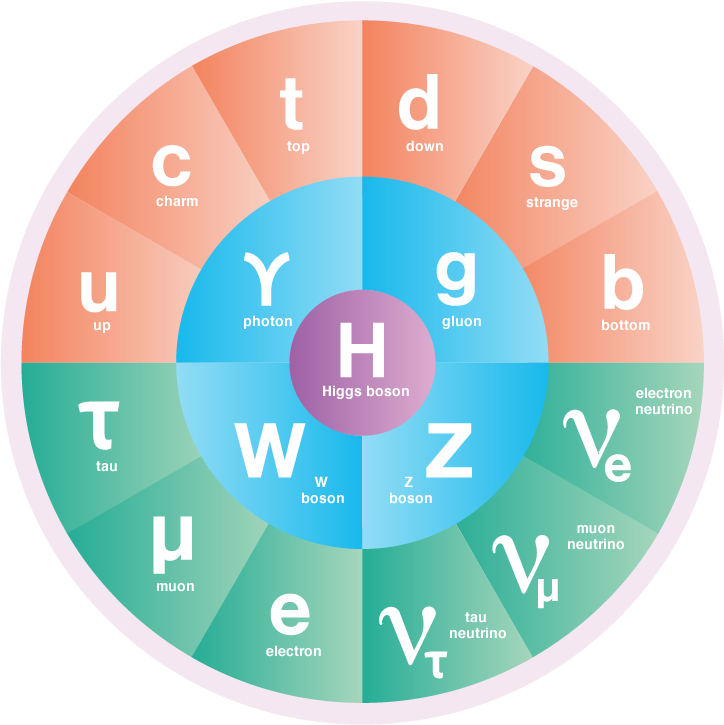
\includegraphics[width=\textwidth]{standard_model}
  \caption[][14.2em]{%
    The particles of the \gls{sm} are divided into subsets:
    quarks (orange), leptons (green), gauge bosons (blue) and the Higgos boson (violet).
    The up-like quarks ($u, c, t$) carry a charge of $\frac{2}{3}e$, while the down-like quarks' ($d, s, b$) charge is $-\frac{1}{3}e$.
    The three leptons on the left ($e, \mu, \tau$) have the charge $-e$, while the leptons on the right ($\nu_e, \nu_\mu, \nu_\tau$) are neutral.
    The gauge bosons are the mediators of electromagnetism ($\gamma$), weak interaction ($W^\pm, Z$) and strong interaction ($g$).
    The Higgs boson ($H$) is reponsible for the \gls{sm} fermions' mass.
    -- \copyright \href{http://www.symmetrymagazine.org/standard-model/}{symmetrymagazine.org}
  }
  \label{fig:standard_model}
\end{figure}

Mathematically speaking, the \gls{sm} is a gauge quantum field theory built upon internal symmetries of the unitary product group $SU(3) \times SU(2) \times U(1)$\marginnote{Unitary and special unitary groups of degree 1, 2 and 3}.

\subsection{The neutrino, from proposal to discovery}
Pauli proposed the existence of a neutral particle with almost no mass in 1930\cite{Brown:1978} to describe the continuous energy spectrum of $\beta$-decays without breaking the principle of energy conservation.
His spin $\frac{1}{2}$, neutral, light particle was practically undetectable, such that he considered his idea not to be in stage of publication.
Enrico Fermi developed a theory of $\beta$-decays based on Pauli's idea and introduced the name neutrino.
Supported by Fermi's theory, Pauli presented his idea in 1933.

The experimental proof of the existence of the neutrino was provided in 1956\marginnote{It took 23 years to proof the existence of neutrinos!} by Frederick Reines' and Clyde L. Cowan, Jr.'s.
The setup consisted of water tanks, liquid scintillator, photomultipliers, an efficient neutron absorber and some logic signal treatment.
Measuring a very characteristic signature of the inverse $\beta$-decay, led to a drastical reduction of the background\cite[-2.5em]{Reines:1995:NobelLecture}.
This made it possible to get significant results, placing the setup close to a nuclear reactor.

\begin{figure*}
  \centering
  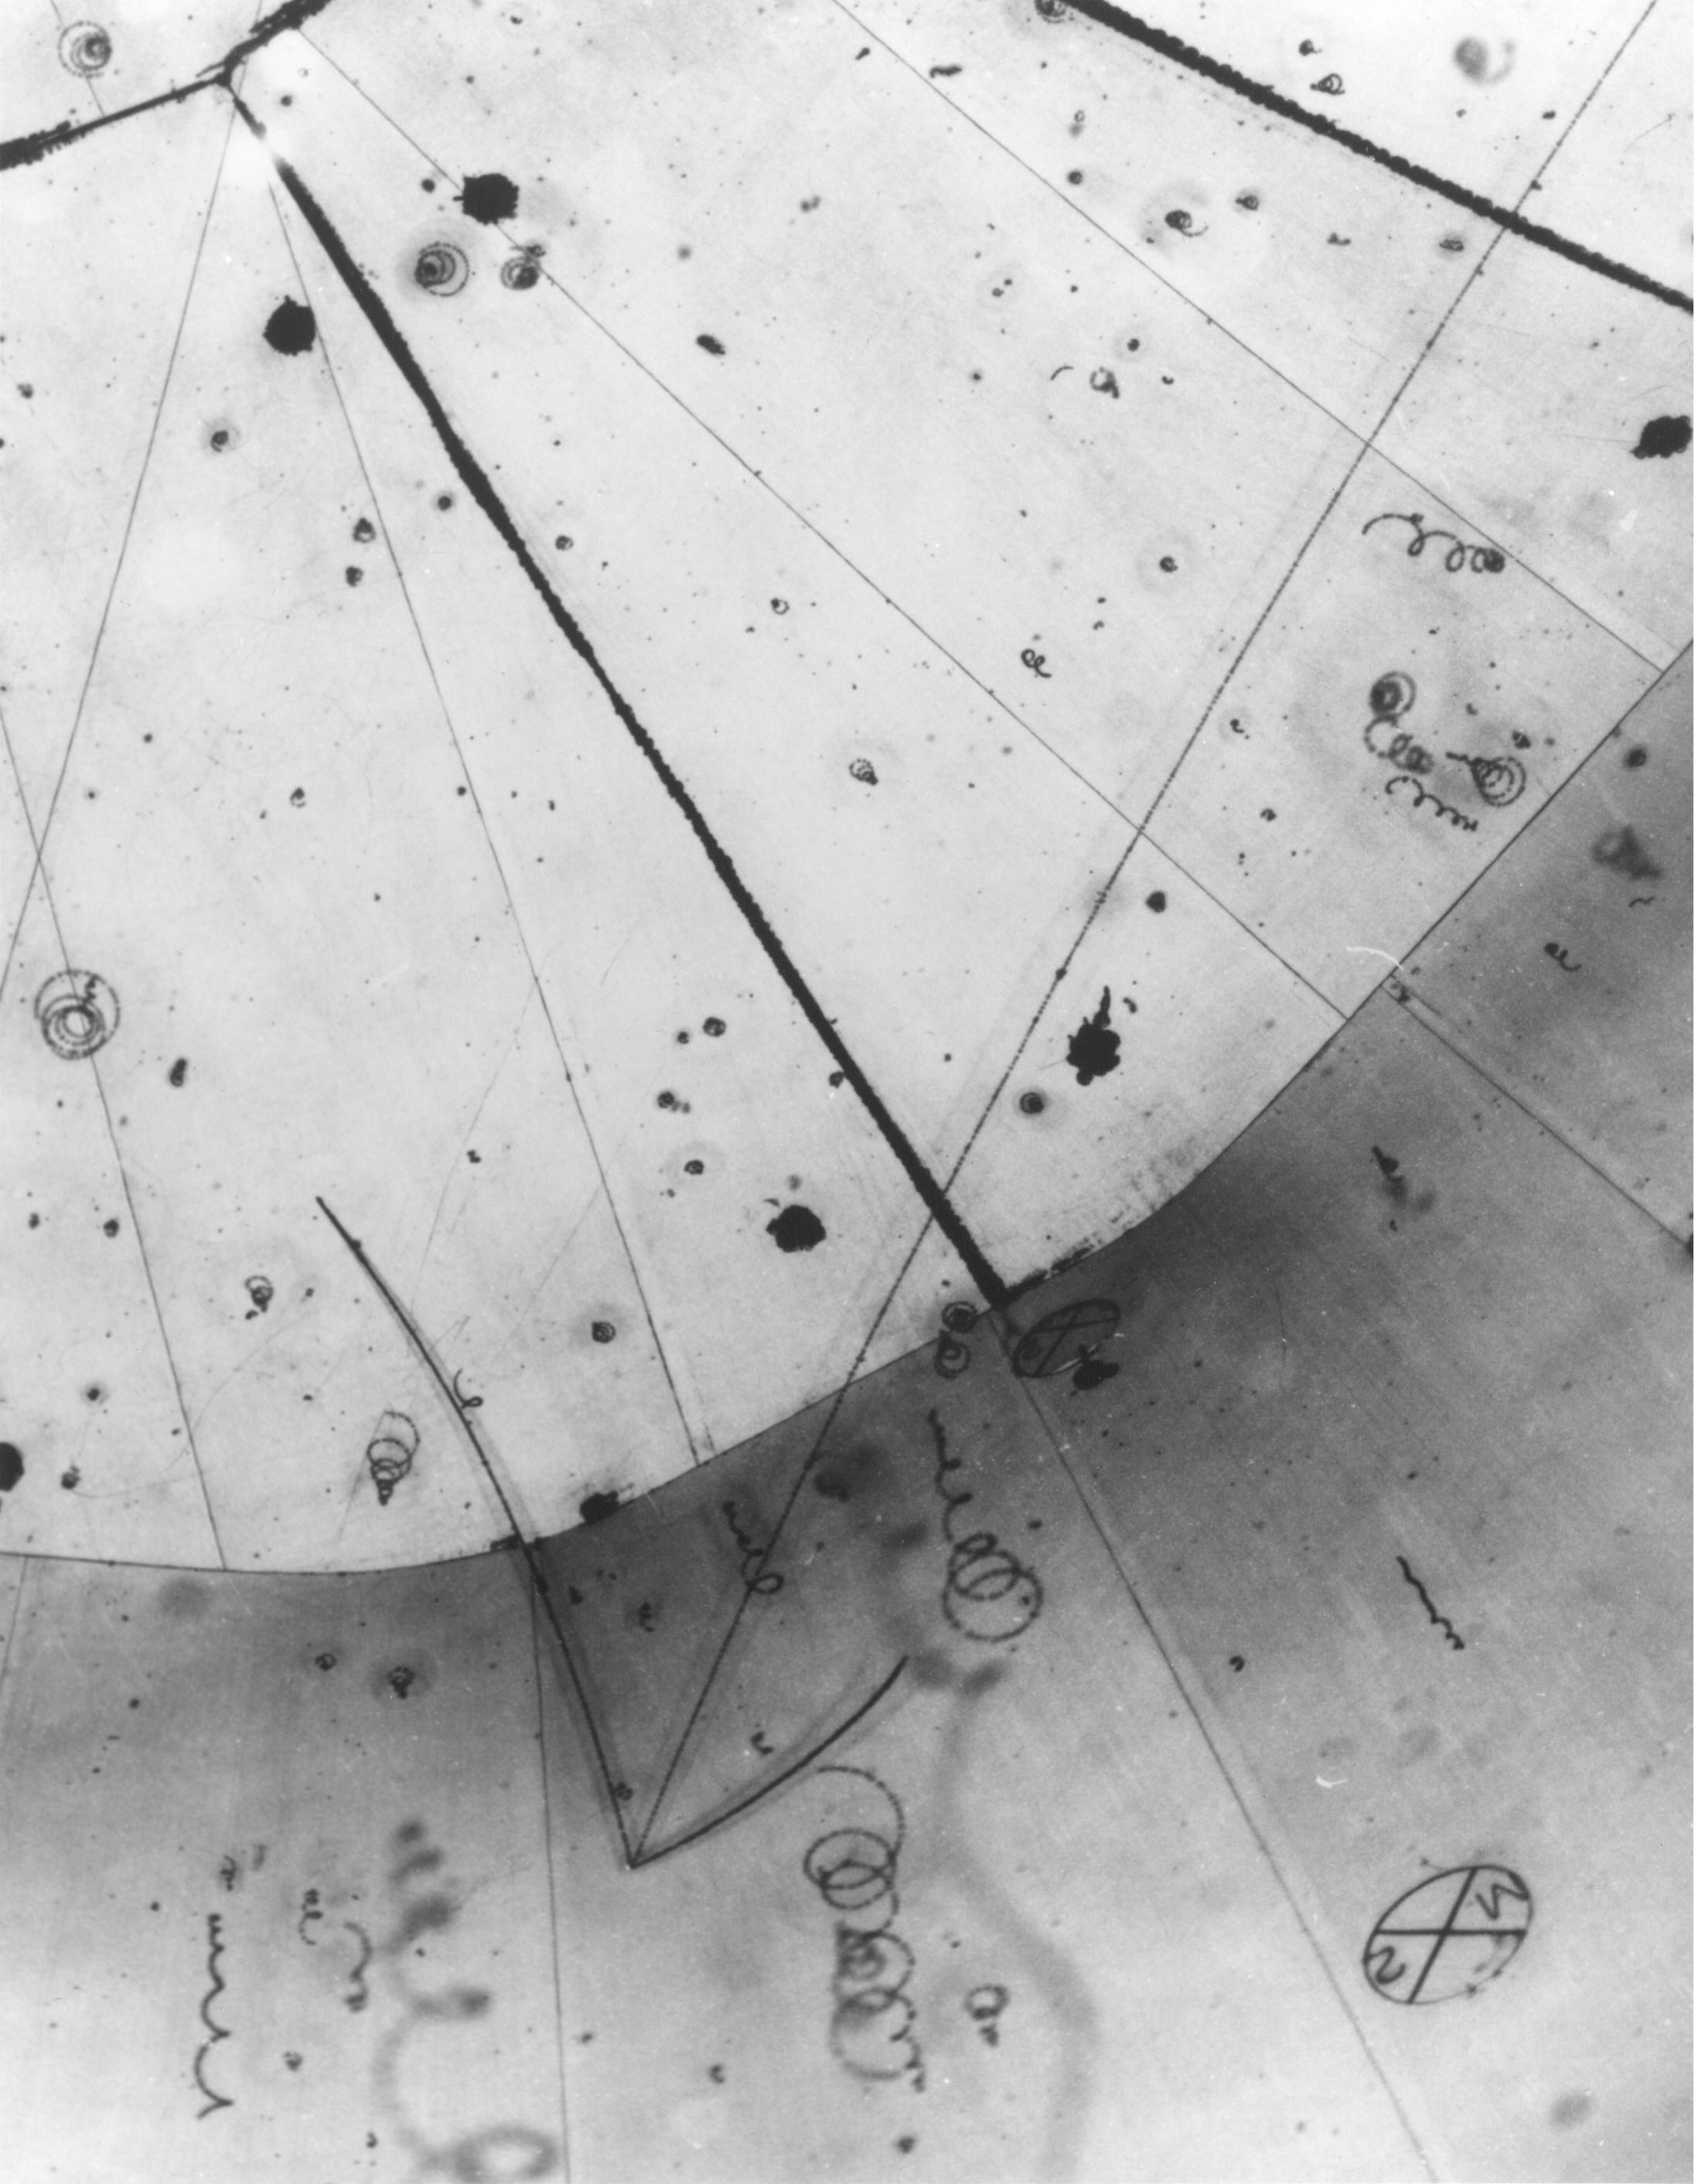
\includegraphics[width=.8\textwidth]{observation}
  \caption[][1em]{%
      World's first neutrino observation (Nov. 13th 1970)
      -- \copyright Argonne National Laboratory
  }
  \label{fig:observation}
\end{figure*}

The Argonne National Laboratory run the Zero Gradient Synchrotron from 1963 to 1979 and used a 12-foot hydrogen bubble chamber to record events from the accelerated particles and their byproducts.
Using this technology, it was possible to register the world's first neutrino observation on November 13th 1970, displayed in figure \ref{fig:observation}.
This event is the irrefutable proof of neutrino's existence.


\subsection{What are neutrino's properties?}
Despite the development of neutrino detectors over the last decades, some neutrino properties remain yet unknown.
Studying the properties of a particle is a good way to check our model's consistency or lead us to new, unknown physics.
This is a good reason to keep developing and running neutrino experiments.

\paragraph{Classification in the \gls{sm}} As proposed by Pauli, neutrinos are neutral particles of small mass with spin 1/2 and therefore fermions.
Neutrinos conserve leptonic number, making them part of the group of leptons.
Neutrinos come in 3 different flavors, and each flavor is associated to one of the heavier leptons: electron neutrino $\nu_e$, muon neutrino $\nu_\mu$ and tauon neutrino $\nu_\tau$.
The number of different light neutrino types was determined by studying Z-Boson production and decay\cite{Karlen:2004fj}.

\paragraph{Helicity} A handy way to group particles is by projecting a particle's spin along its direction of motion getting as a result its helicity.
Particles with a positive helicity are called right-handed, their counterpart is called left-handed.
So far there's no experimental evidence for right-handed neutrinos or left-handed antineutrinos\cite{1601.00627}\cite{Romero:2016str}.
The first hints for neutrino's helicity were given T.D. Lee and C.N. Yang.
They predicted in 1956 parity violation in weak interactions, by expressing the weak interaction as a chiral gauge interaction.
This was later shown by Chien-Shiung Wu in collaboration with the Low Temperature Group of the US National Bureau of Standards\cite{PhysRev.105.1413}.

\paragraph{Mass} Bruno Pontecorvo and Vladimir Gribov had an idea\marginnote{further developed by Ziro Maki, Masami Nakagawa and Shoichi Sakata}, which predicted that neutrinos undergo changes in flavor, called neutrino oscillations\cite{Bahcall:2004}.
Raymond Davis Jr. and John Bahcall's solar neutrino problem strongly indicated the existence of neutrino oscillations and Takaaki Kajita and Arthur B. McDonald confirmed this with their experiment.
Neutrino oscillations require neutrinos to have a non-zero mass and allow to study neutrino's relative mass.\marginnote{The \gls{sm} gives mass to fermions by the interaction with the Higgs field, which involves interactions with particles of both chiralities.
Since no right-handed neutrinos and left-handed antineutrinos were observed so far, it is not clear where the neutrino masses arise from.}
On the other hand the absolute mass of the three flavors of neutrinos remains unknown, such that different hierarchies are possible.
At the point of writing, two possible hierarchies are considered: the normal hierarchy and the inverted hierarchy.

\paragraph{Neutrino velocities} Due to their small mass, neutrinos generated in particle physics processes are expected to have velocities close to the one of light in vacuum\marginnote{So called hot matter}.
The velocity of neutrinos was measured in several experiments, confirming the theory's expectations\cite{Antonello:2012be}\cite{Adam:2011faa}.

